\documentclass[11pt]{beamer}
\usetheme{Singapore}
\usepackage[utf8]{inputenc}
\usepackage[french]{babel}
\usepackage[T1]{fontenc}
\usepackage{amsmath}
\usepackage{amsfonts}
\usepackage{amssymb}
\author{Le groupe MkRpg}
\title{Présentation du projet MkRpg}
%\setbeamercovered{transparent} 
\setbeamertemplate{navigation symbols}{} 
\renewcommand{\insertnavigation}[1]{\hfill
\includegraphics[scale=.5]{main.png}~\vspace{-.2cm}}
% Raoul :
%\renewcommand{\insertnavigation}[1]{\hfill
\includegraphics[scale=.25]{raoul.png}~\vspace{-.2cm}}
%\setbeamertemplate{headline}{}
%\logo{} 
%\institute{} 
%\date{} 
%\subject{} 
\begin{document}

\begin{frame}
\titlepage
\end{frame}

\begin{frame}{Sommaire}
\tableofcontents
\end{frame}

\section{Éditeur}

\subsection{Objectifs}
\begin{frame}{Objectifs}
\begin{itemize}
\item Création des jeux
\item Modification de jeux
\item Création de XML pour le serveur et les clients
\item Utilisation d'abstractions pour l'édition (Ajout de vie, déroulement du temps, ...)
\end{itemize}
\end{frame}



\subsection{Choix techniques}

\begin{frame}{Outils utilisés}

\textbf{Langage de programmation :}
C++
\begin{itemize}
\item Sécurité et confort du typage
\item Performances
\item Lisibilité du code (.h)
\end{itemize}

~


\textbf{Interface graphique :}
Framework Qt

\begin{itemize}
\item Connaissances préalables
\item Outils de création de fenêtre puissant (Qt Designer)
\item API haut niveau (lecture/écriture XML)
\end{itemize}

~

\textbf{Inconvénients :} Duplication de code
\end{frame}


\subsection{Architecture}

\begin{frame}{Architecture}
\textbf{Architecture globale :}
\begin{itemize}
\item Modèle :
\begin{itemize}
\item Représentation interne des données
\item Accesseurs et mutateurs pour assurer des invariants
\end{itemize}
\item Interface :
\begin{itemize}
\item Accès au données
\item Abstraction des mécanismes d'événements et d'actions
\end{itemize}
\end{itemize}

\end{frame}

\begin{frame}{Interface}

\textbf{Architecture Qt classique}
\begin{itemize}
\item Sous classe pour les \textit{widgets} d'affichage spécifiques
\item Utilisation de l'API Model/View
\end{itemize}

~

\textbf{Éditeurs spécifiques aux objets}

Patron de conception \textit{fabrique}

\end{frame}


\begin{frame}{Modèle}


\textbf{Classe de base : } \texttt{GameObject} 
\begin{itemize}
\item Utilisation du polymorphisme (écriture de XML, édition)
\item Organisation des jeux en arbre
\item Éléments communs : 
\begin{itemize}
\item Paramètres
\item Drapeaux
\item Événements
\item Ordres
\end{itemize}
\item Mécanismes d'information des modifications
\item Facilité de libération de mémoire
\item Identifiant unique
\end{itemize}


\end{frame}
\begin{frame}{Modèle}

\textbf{Héritage d'objet}
\begin{itemize}
\item Classe \texttt{InheritableObject}
\item Distinction \texttt{Type/TypedObject}
\item Redéfinition des valeurs des paramètres/drapeaux
\end{itemize}

~

\textbf{Objets virtuels d'organisation :}
\begin{itemize}
\item \texttt{DefaultTypes}
\item \texttt{GameObjectList}
\item \texttt{GameObjectInventory}
\end{itemize}

\end{frame}


\begin{frame}{Modèle}
\textbf{Diagramme des classes}

~

\begin{center}
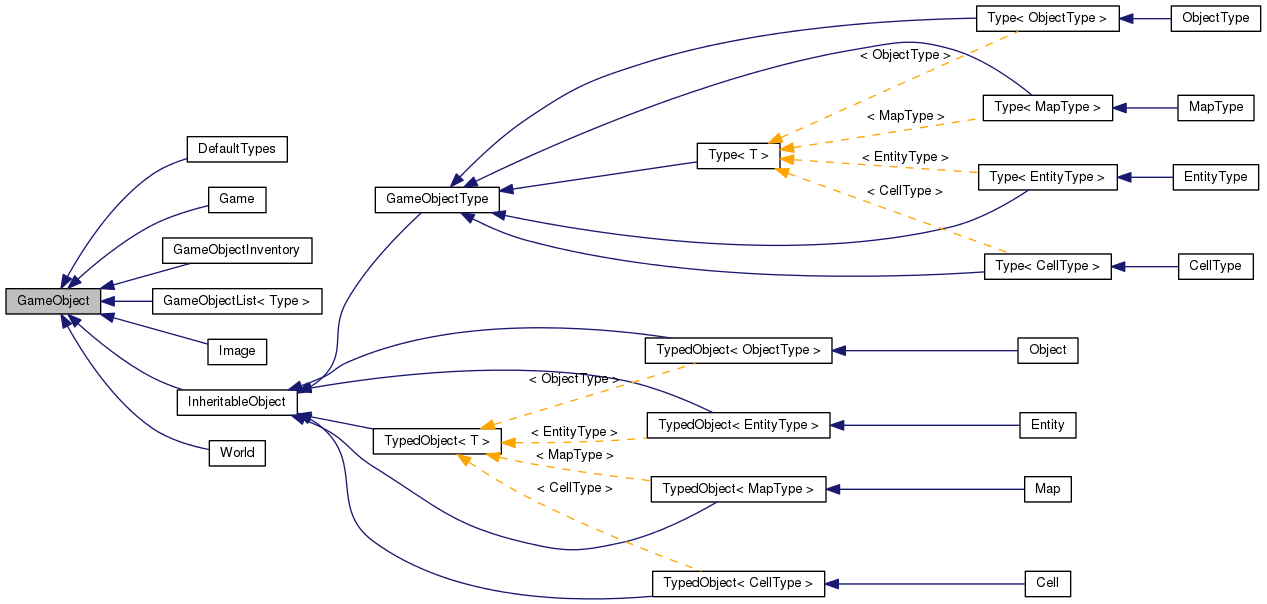
\includegraphics[scale=.24]{GameObject.png}
\end{center}

\end{frame}


\begin{frame}{XML}
\textbf{Export}
\begin{itemize}
\item XML du serveur : lisible par les serveur/clients
\item XML de l'éditeur : contient des informations d'édition et d'organisation interne
\end{itemize}

~

\textbf{Import}

Import de jeux par lecture de XML (éditeur)

\end{frame}


\section{Commentaires}
\begin{frame}{Difficultés - Choix discutables \textit{a posteriori}}

\begin{itemize}
\item Préciser les architectures avant de coder
\item Choix d'outils : éviter de re-coder la roue
\item Faire avancer les différents composants à la même vitesse
\end{itemize}

\end{frame}


\begin{frame}{Perspectives}
\begin{itemize}
\item Définition d'un langage d'ordre
\item Ajout d'abstractions dans l'éditeur
\item Révisions du XML (pour que XML serveur $\subset$ XML éditeur)
\end{itemize}
\end{frame}

\end{document}
